% !Mode:: "TeX:UTF-8"

\chapter{数据处理}

\section{数据预览}

船舶图像:(19万张左右)

\begin{figure}
\centering
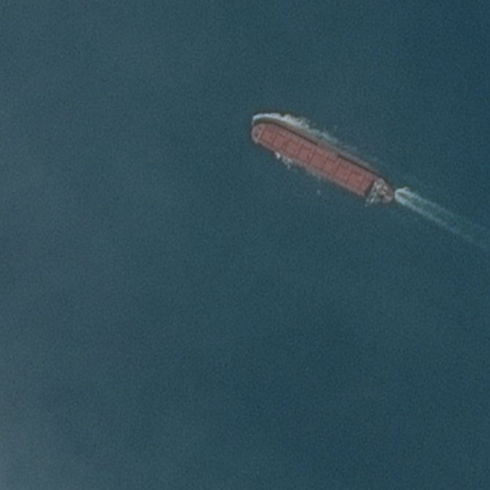
\includegraphics{body/model_pic/boat_example}
\caption{}
\end{figure}

数据目标:(保存在csv表格中)

\begin{figure}
\centering
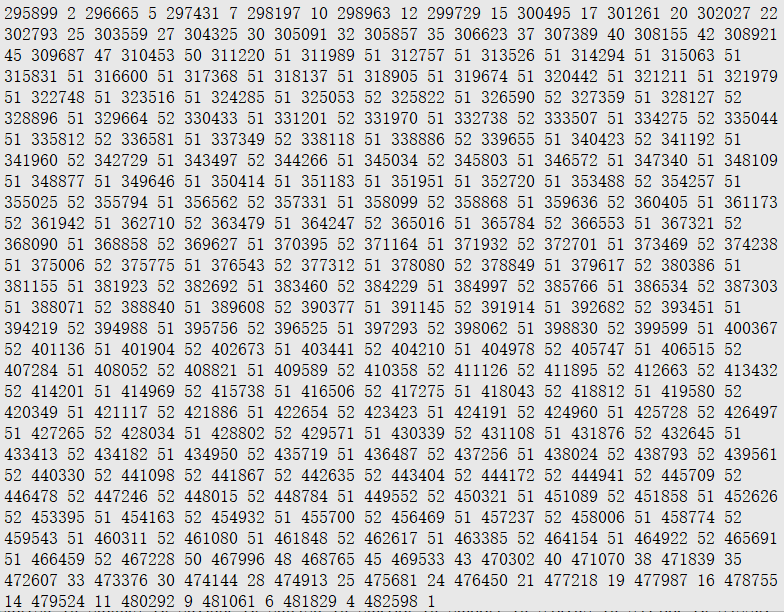
\includegraphics{body/model_pic/target_example}
\caption{}
\end{figure}

这是所得数据的rle编码,解码效果如下:

\begin{figure}
\centering
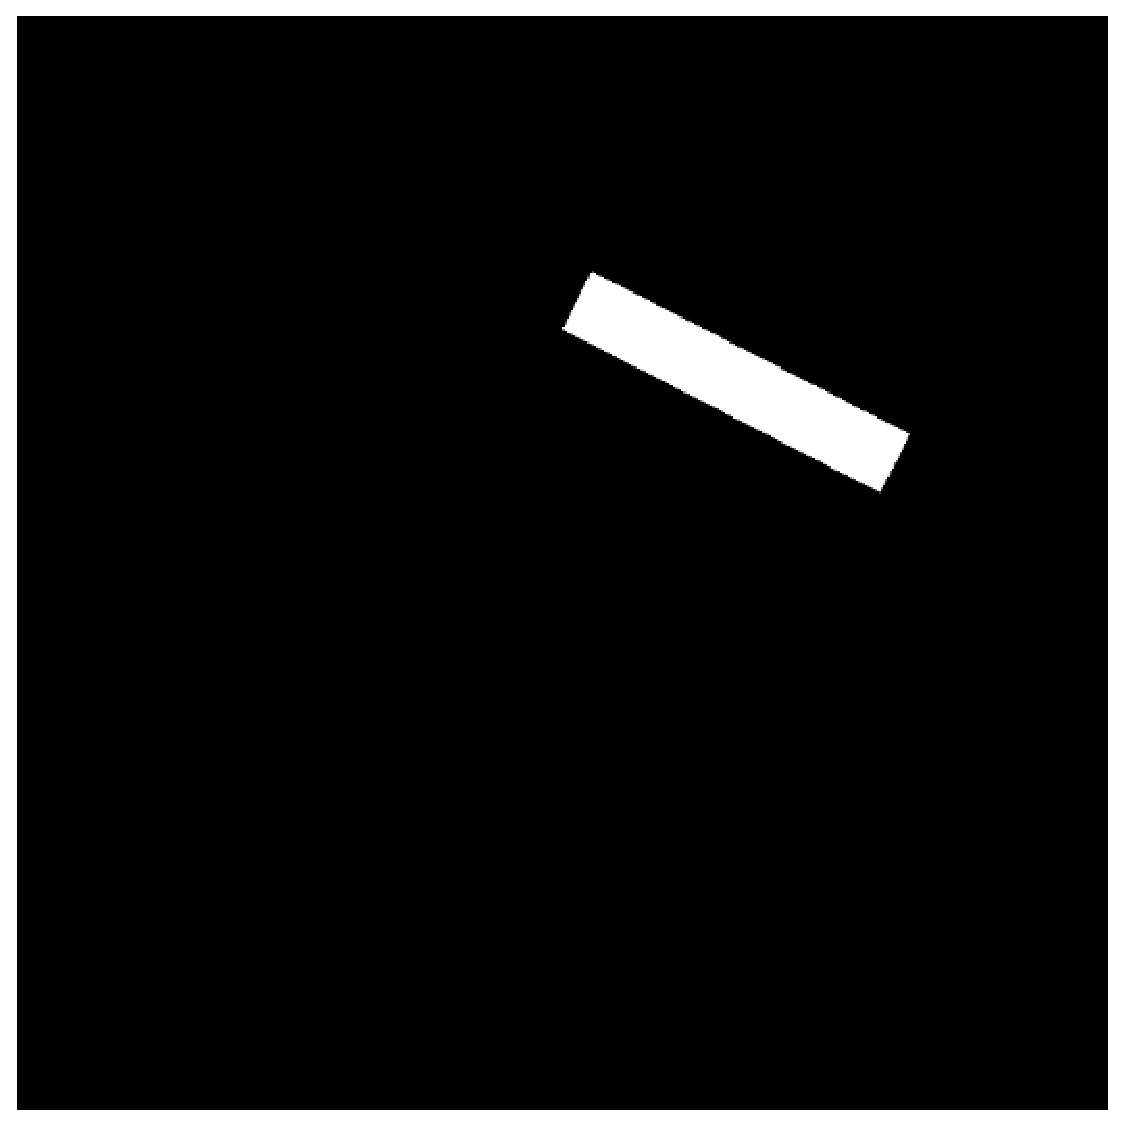
\includegraphics{body/model_pic/rle_decode}
\caption{}
\end{figure}

\section{数据解码}

Rle编码(Run Length
Encoding),它的原理是通过检测统计数据流中重复的位或字符序列,并用它们出现的次数和每次出现的个数形成新的代码。从而达到数据压缩的目的。

例如,``5 3 10
4''表示,目标所在位置包括:第5个像素点开始连续的3个像素点和第10个像素点开始连续的4个像素点。

Rle解码算法:

新建一张全0图像,对其修改对应的目标像素为1。

Rle解码代码如下:

\begin{verbatim}
def rle_to_array(img, rles):
    l, w = img.shape[0], img.shape[1]
    x = np.asarray(img).reshape((l, w, 3))
    y = np.zeros(l * w, dtype=np.uint8)

    for rle in rles.values:
        if rle is np.nan:
            break
        rle = rle.split(' ')
        starts, lengths = [np.asarray(x, dtype=int) for x in (rle[0:][::2], rle[1:][::2])]
        starts -= 1
        ends = starts + lengths
        for s, e in zip(starts, ends):
            y[s:e] = 1

    y = y.reshape((l, w)).T.reshape((l, w, 1))
    return x, y
\end{verbatim}

\section{数据清洗}

删除数据中的残缺图像、模糊图像、重复图像。

\begin{figure}
\centering

\includegraphics{body/model_pic/bad_image1}
\caption{}
\end{figure}

\begin{figure}
\centering
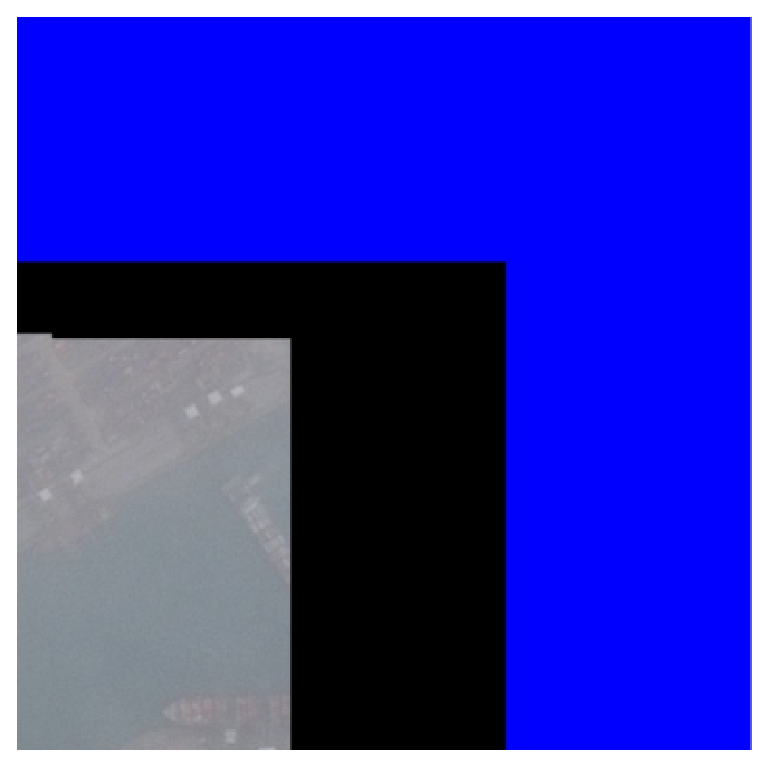
\includegraphics{body/model_pic/bad_image2}
\caption{}
\end{figure}

\begin{figure}
\centering
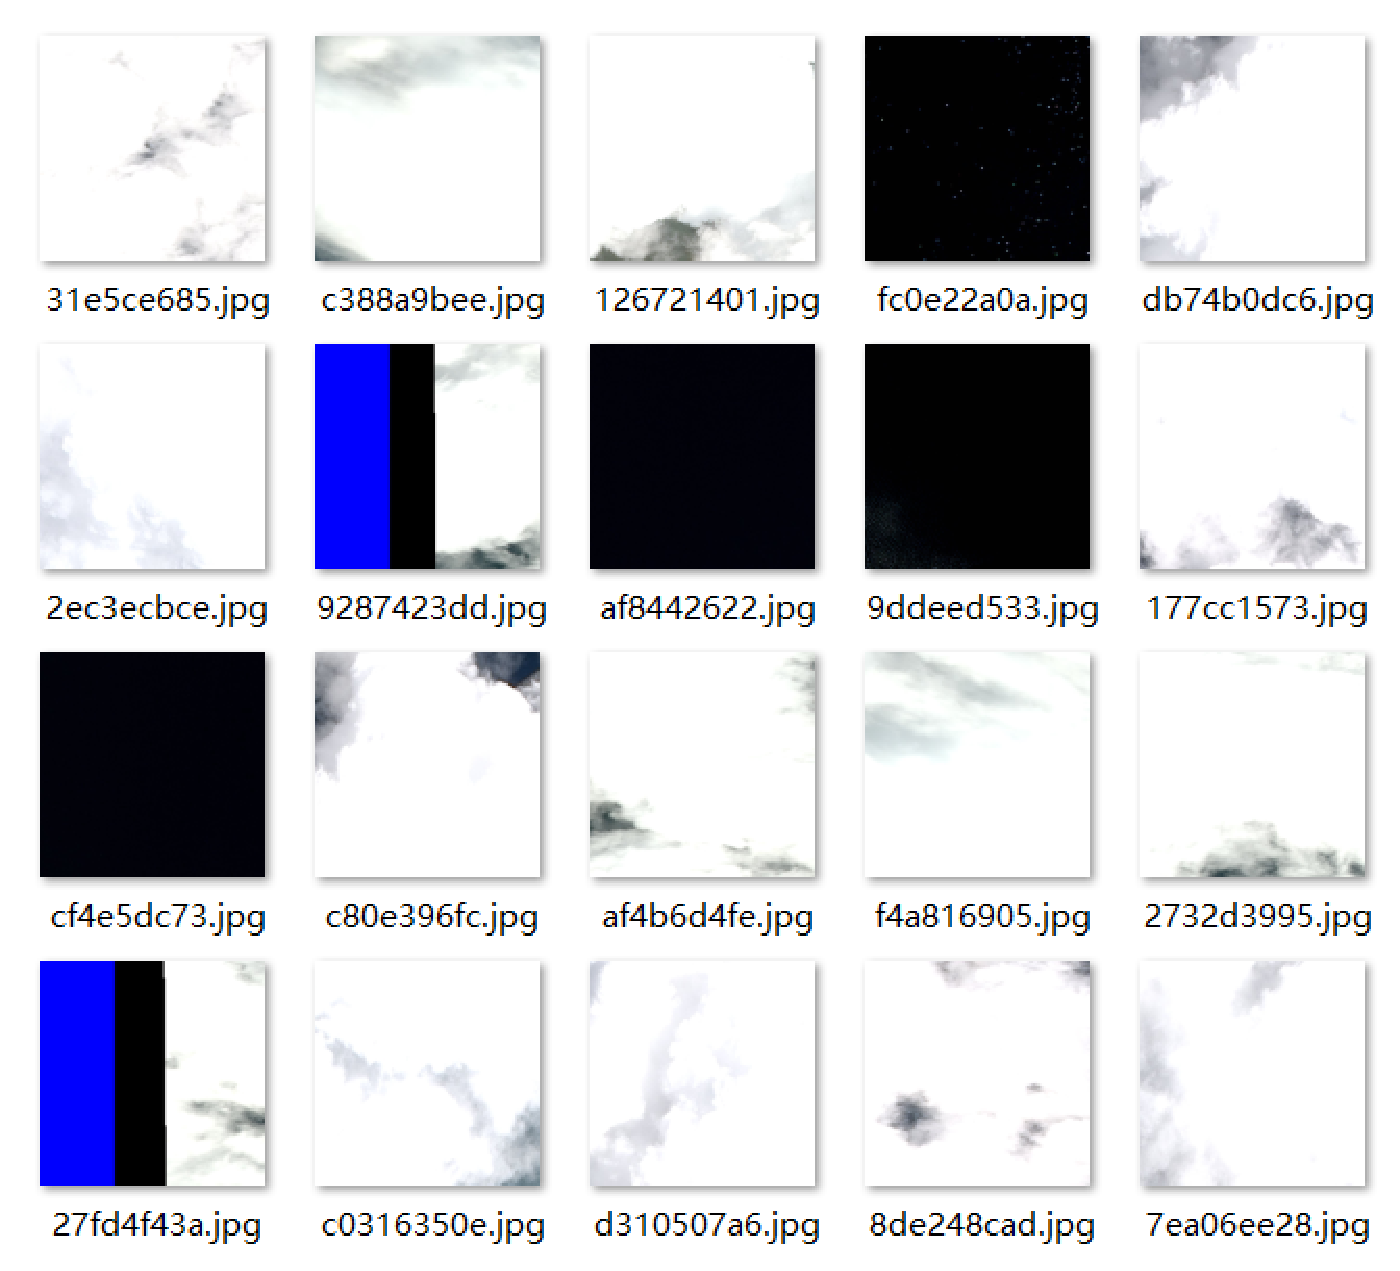
\includegraphics{body/model_pic/bad_image3}
\caption{}
\end{figure}

对粘连的小船舶数据,实行部分舍弃或合并。

\begin{figure}
\centering
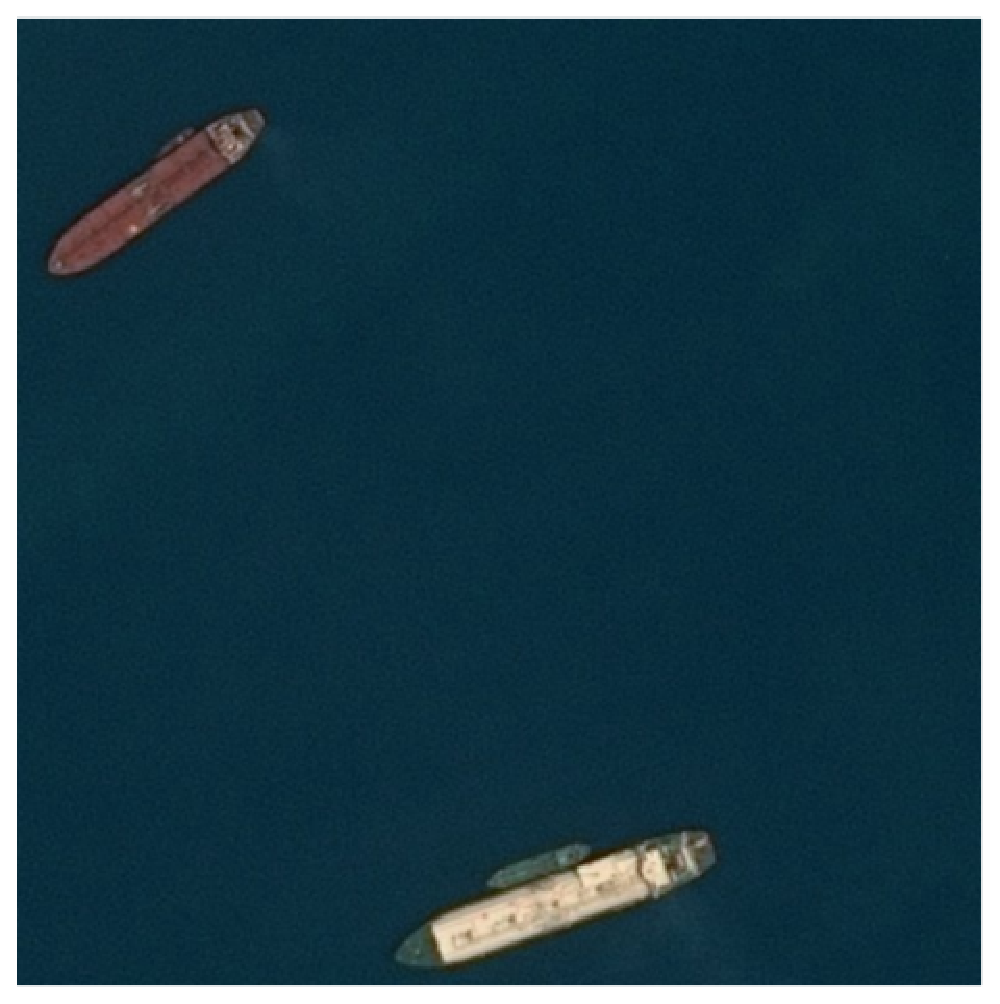
\includegraphics{body/model_pic/bad_image4}
\caption{}
\end{figure}

\section{数据平衡}

由于图像中的船只数量并不固定,因此我们将其分类:

\subsection{先按照有无船只分类}

\begin{figure}
\centering
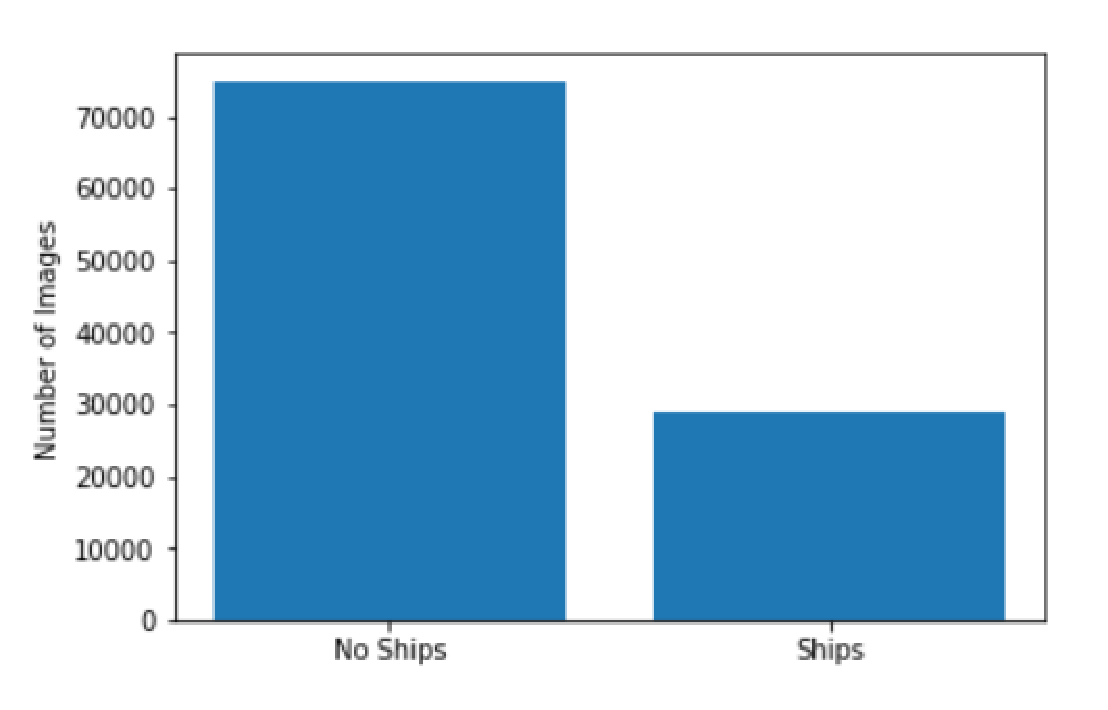
\includegraphics{body/model_pic/noship_ship}
\caption{}
\end{figure}

无船图像大概有15万张,有船图像大概有4万张。

\begin{figure}
\centering
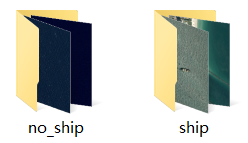
\includegraphics{body/model_pic/noship_ship_dir}
\caption{}
\end{figure}

\begin{figure}
\centering
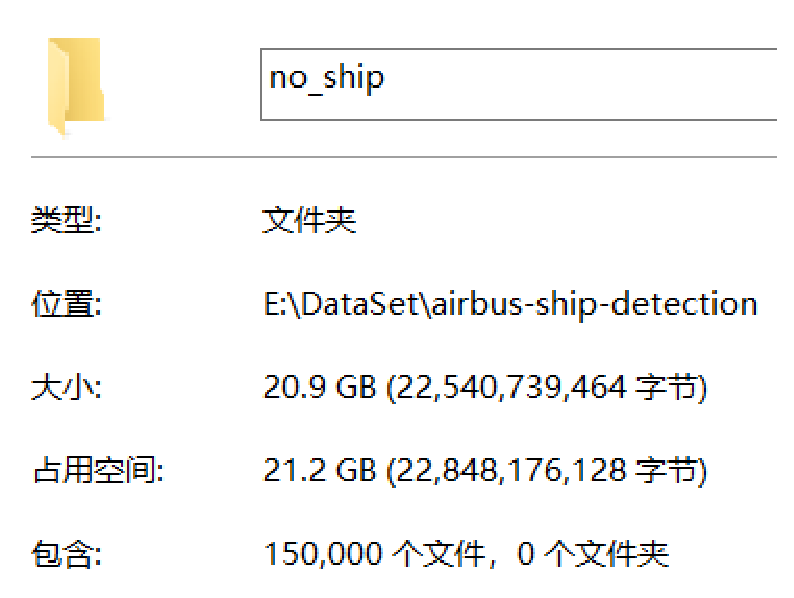
\includegraphics{body/model_pic/no_ship}
\caption{}
\end{figure}

\begin{figure}
\centering
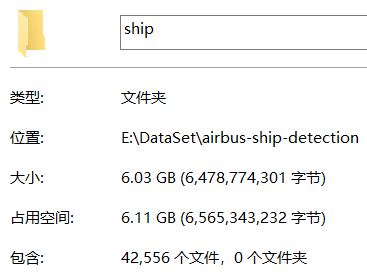
\includegraphics{body/model_pic/ship}
\caption{}
\end{figure}

\subsection{再根据船只数量分类}

\begin{figure}
\centering
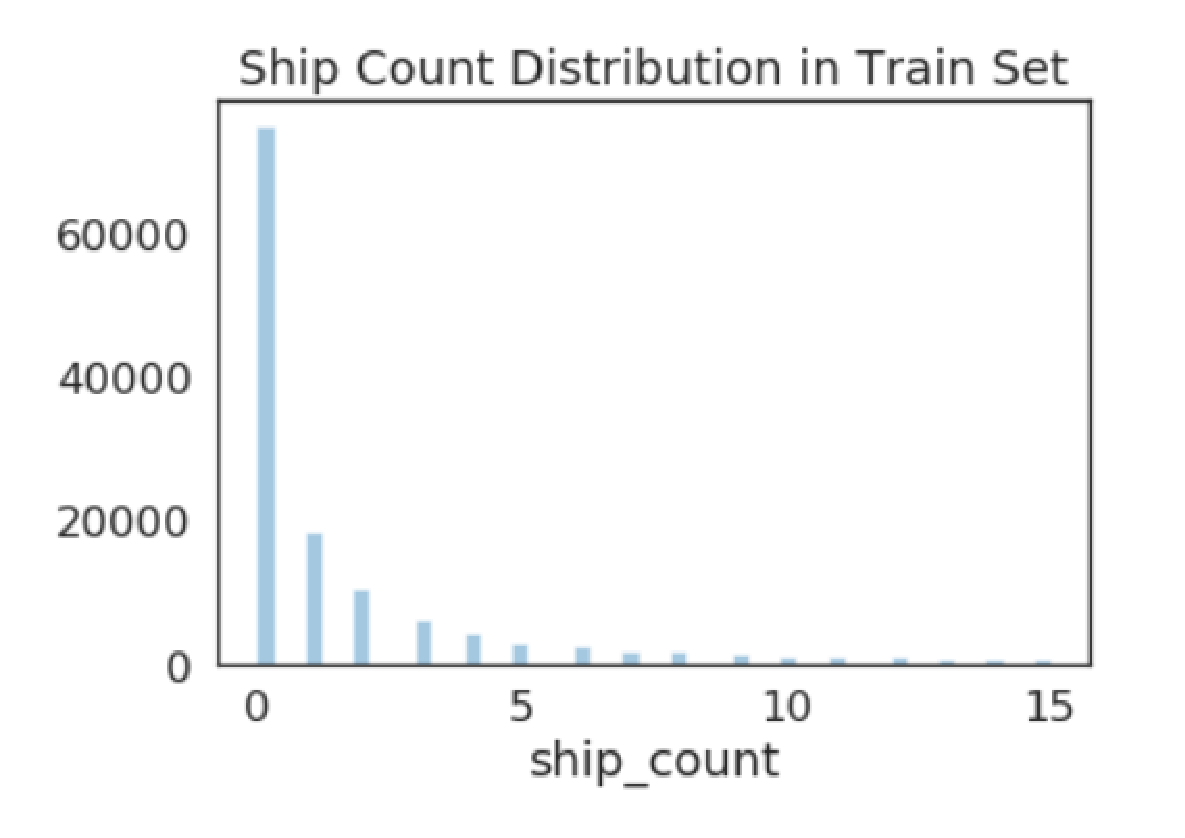
\includegraphics{body/model_pic/count_boat}
\caption{}
\end{figure}

特点为:图像中船只数量越多,图像数量越少。

\subsection{将不同船只数量的图像按比例结合}

将每种图像都取出一部分放入预准备数据中,使各种数据比例大致相同,得到一个平衡的预准备数据。(无船图像数据中包含内容较少,不取)

\section{数据生成}

由于原始数据是RGB图像数据,所占内存较大,为了防止内存溢出,制作一个数据生成器。

定义一个循环,不断地用随机数选择图像数据,选择后将目标数据进行解码处理得到L图像数据,最后将RGB图像和L图像抛出。

代码如下:

\begin{verbatim}
def generator(imgs, results, batch_size, seed=None):
    if seed:
        np.random.seed(seed)
    ImageId, EncodedPixels = results["ImageId"], results["EncodedPixels"]
    while True:
        samples = np.random.choice(imgs, size=batch_size)
        X, Y = [], []
        for s in samples:
            img = Image.open(img_path)
            rles = EncodedPixels[ImageId == s]
            x, y = rle_to_array(img, rles)
            X.append(x)
            Y.append(y)
        X, Y = np.asarray(X) / 255, np.asarray(Y)
        yield (X, Y)
\end{verbatim}

\section{数据增强}

使用keras库的ImageDataGenerator,设置多种参数使图像进行各种变换而产生更多的数据。

常用参数设置:

\begin{longtable}[]{@{}cc@{}}
\toprule
参数 & 功能\tabularnewline
\midrule
\endhead
Rotation\_range & 图像随即旋转的角度范围\tabularnewline
width\_shift/height\_shift &
图像在水平或垂直方向上的平移范围\tabularnewline
Shear\_range & 随机错切变换的范围\tabularnewline
Zoom\_range & 图像随机缩放的范围\tabularnewline
Horizontal\_flip & 随机将一半图像水平翻转\tabularnewline
Fill\_mode & 用于填充新创建像素的方法\tabularnewline
\bottomrule
\end{longtable}

例:

\begin{figure}
\centering
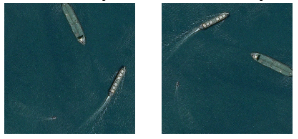
\includegraphics{body/model_pic/change1}
\caption{}
\end{figure}

\begin{figure}
\centering
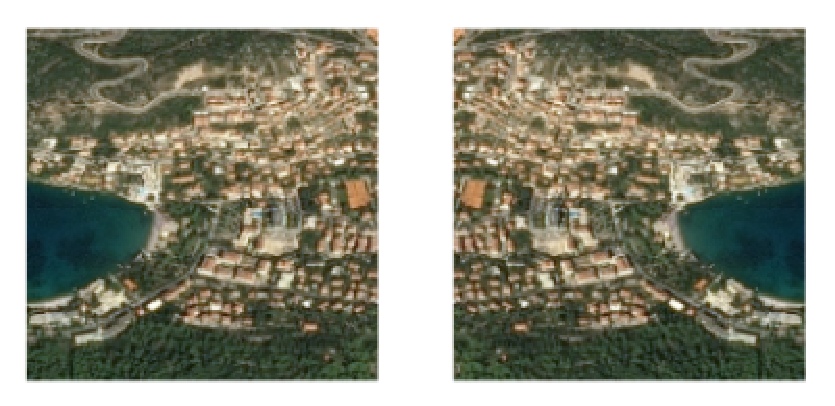
\includegraphics{body/model_pic/change2}
\caption{}
\end{figure}

\chapter{模型建立}

\section{U-net简介}

\begin{figure}
\centering
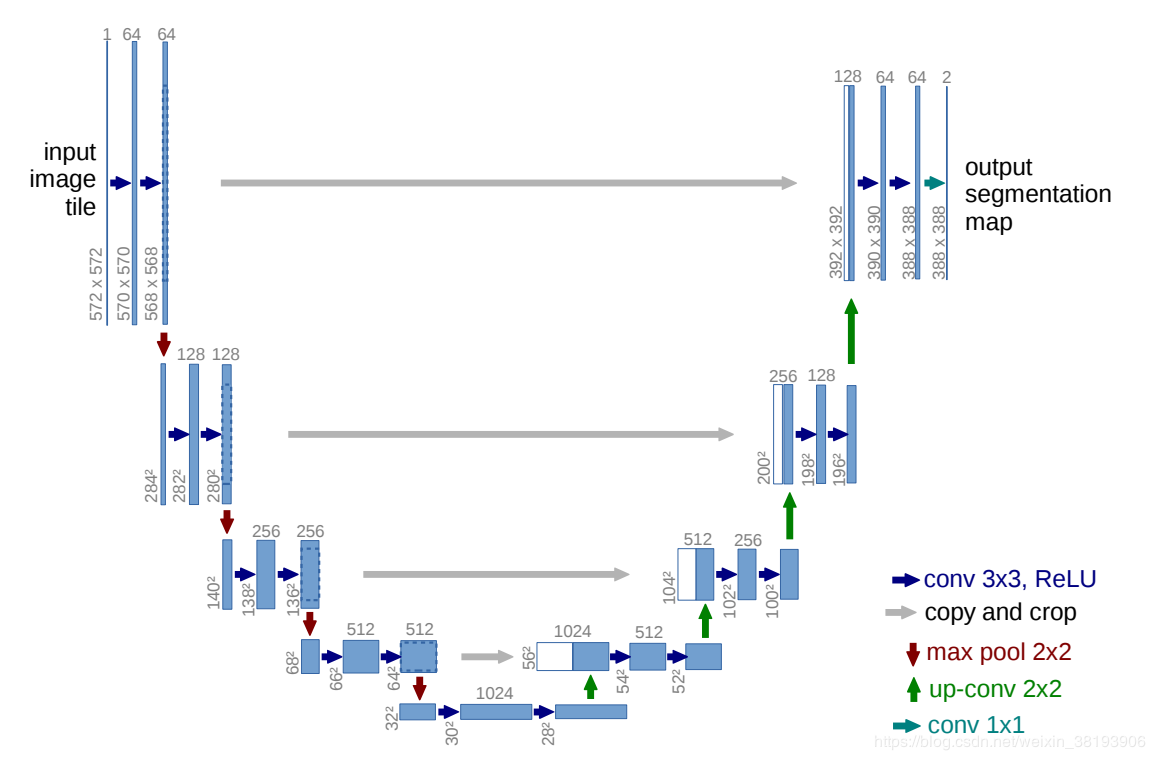
\includegraphics{body/model_pic/unet}
\caption{}
\end{figure}

模型的结构十分的对称,左边为一系列连续地卷积池化,而右边则相反,为一系列连续地上采样卷积,而图中灰色箭头则是残差连接,将浅层特征与深层特征结合,避免了特征的损失,此模型因结构形似``U''形,而被称为U-net。

\section{模型搭建}

\subsection{卷积池化}

\begin{verbatim}
c = Conv2D(8, (3, 3), activation='relu', padding='same')(x)
c = Conv2D(8, (3, 3), activation='relu', padding='same')(c)
p = MaxPooling2D((2, 2))(c)
\end{verbatim}

\subsection{拼接+反卷积}

\begin{verbatim}
c2 = Conv2DTranspose(8, (2, 2), strides=(2, 2), padding='same')(c)
m = concatenate([c1, c2], axis=3)
c = Conv2D(8, (3, 3), activation='relu', padding='same')(m)
c = Conv2D(8, (3, 3), activation='relu', padding='same')(c)
\end{verbatim}

Conv2DTranspose可用UpSampling2D+Conv2D代替。

\subsection{添加批标准化层}

\begin{verbatim}
c = BatchNormalization()(c)
\end{verbatim}

统一分布,加强网络的泛化能力;

使用更高的学习率,加快训练速度;

充当Dropout,防止过拟合。

\subsection{优化器与损失}

optimizer使用Adam优化器,loss取(1-IoU),IoU是预测图像与真实图像的重合率,IoU越大,loss越小。

\begin{figure}
\centering
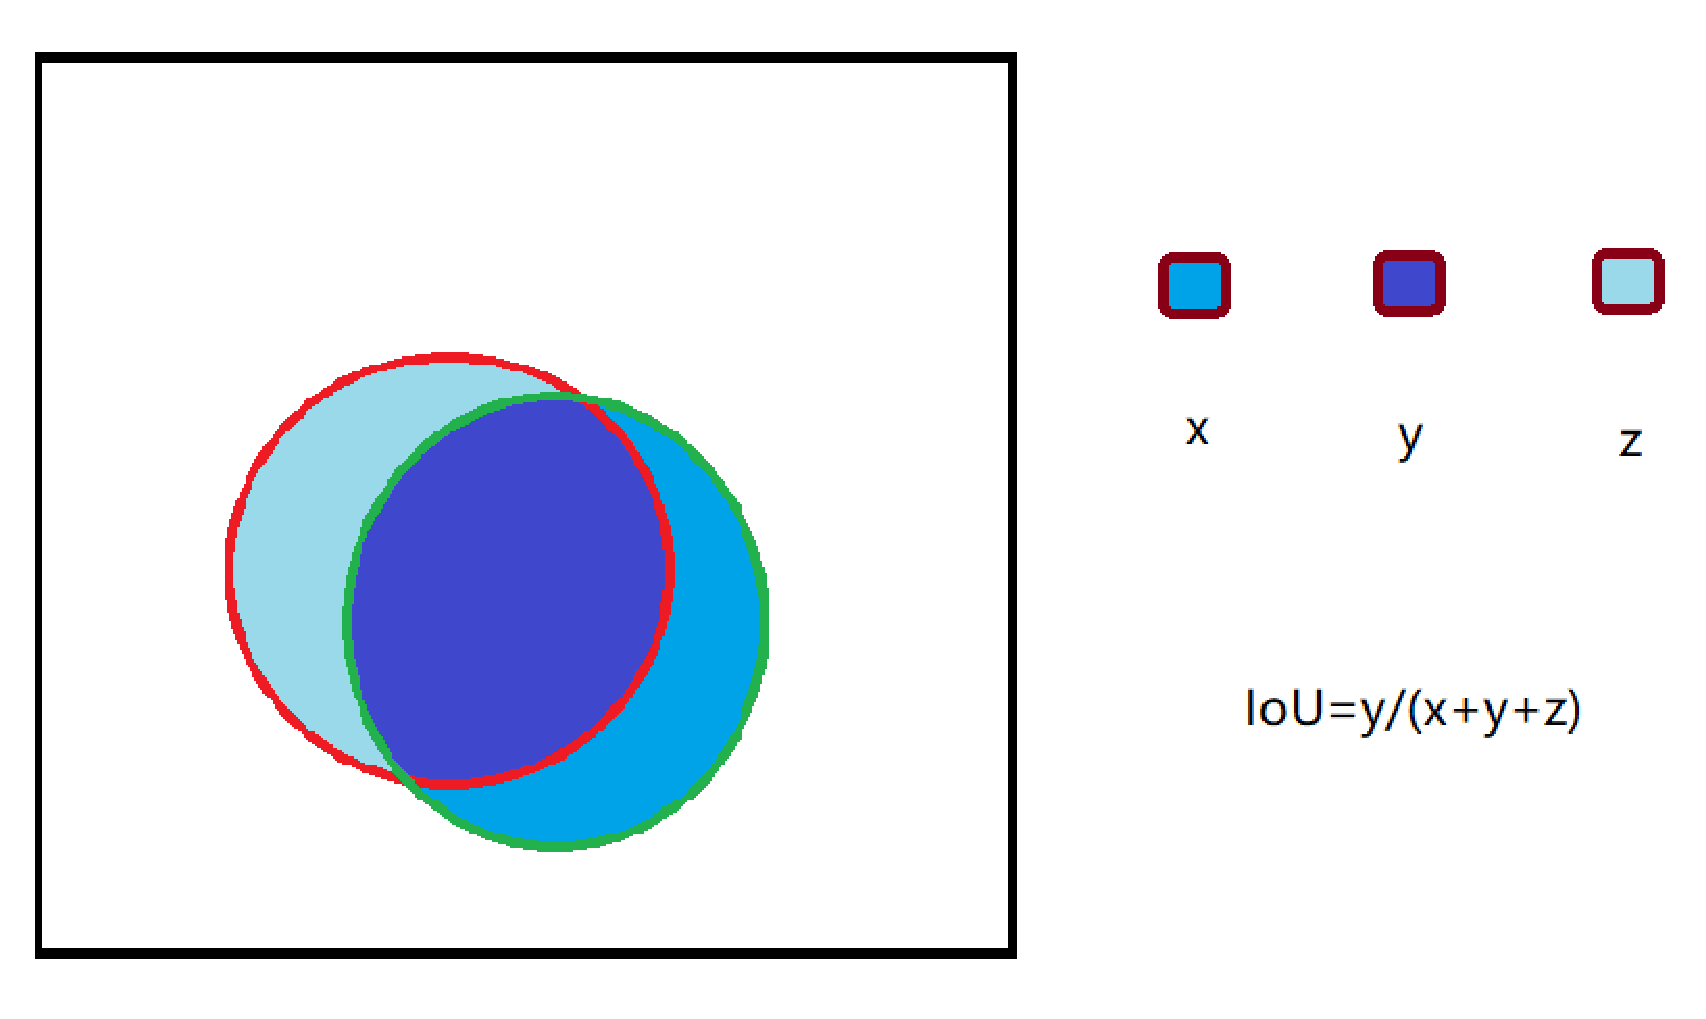
\includegraphics{body/model_pic/iou}
\caption{}
\end{figure}

\subsection{输入输出}

\begin{verbatim}
input = Input((512, 512, 3))
output = Conv2D(1, (1, 1), activation='sigmoid')(c)
\end{verbatim}

输入RGB图像,输出01图像,实质是像素点矩阵。

\subsection{模型结果}

\begin{verbatim}
__________________________________________________________________________________________________
Layer (type)                    Output Shape         Param #     Connected to                     
==================================================================================================
input_1 (InputLayer)            (None, 512, 512, 3)  0                                            
__________________________________________________________________________________________________
conv2d_1 (Conv2D)               (None, 512, 512, 8)  224         input_1[0][0]                    
__________________________________________________________________________________________________
batch_normalization_1 (BatchNor (None, 512, 512, 8)  32          conv2d_1[0][0]                   
__________________________________________________________________________________________________
conv2d_2 (Conv2D)               (None, 512, 512, 8)  584         batch_normalization_1[0][0]      
__________________________________________________________________________________________________
batch_normalization_2 (BatchNor (None, 512, 512, 8)  32          conv2d_2[0][0]                   
__________________________________________________________________________________________________
max_pooling2d_1 (MaxPooling2D)  (None, 256, 256, 8)  0           batch_normalization_2[0][0]      
__________________________________________________________________________________________________
conv2d_3 (Conv2D)               (None, 256, 256, 16) 1168        max_pooling2d_1[0][0]            
__________________________________________________________________________________________________
batch_normalization_3 (BatchNor (None, 256, 256, 16) 64          conv2d_3[0][0]                   
__________________________________________________________________________________________________
conv2d_4 (Conv2D)               (None, 256, 256, 16) 2320        batch_normalization_3[0][0]      
__________________________________________________________________________________________________
batch_normalization_4 (BatchNor (None, 256, 256, 16) 64          conv2d_4[0][0]                   
__________________________________________________________________________________________________
max_pooling2d_2 (MaxPooling2D)  (None, 128, 128, 16) 0           batch_normalization_4[0][0]      
__________________________________________________________________________________________________
conv2d_5 (Conv2D)               (None, 128, 128, 32) 4640        max_pooling2d_2[0][0]            
__________________________________________________________________________________________________
batch_normalization_5 (BatchNor (None, 128, 128, 32) 128         conv2d_5[0][0]                   
__________________________________________________________________________________________________
conv2d_6 (Conv2D)               (None, 128, 128, 32) 9248        batch_normalization_5[0][0]      
__________________________________________________________________________________________________
batch_normalization_6 (BatchNor (None, 128, 128, 32) 128         conv2d_6[0][0]                   
__________________________________________________________________________________________________
max_pooling2d_3 (MaxPooling2D)  (None, 64, 64, 32)   0           batch_normalization_6[0][0]      
__________________________________________________________________________________________________
conv2d_7 (Conv2D)               (None, 64, 64, 64)   18496       max_pooling2d_3[0][0]            
__________________________________________________________________________________________________
batch_normalization_7 (BatchNor (None, 64, 64, 64)   256         conv2d_7[0][0]                   
__________________________________________________________________________________________________
conv2d_8 (Conv2D)               (None, 64, 64, 64)   36928       batch_normalization_7[0][0]      
__________________________________________________________________________________________________
batch_normalization_8 (BatchNor (None, 64, 64, 64)   256         conv2d_8[0][0]                   
__________________________________________________________________________________________________
max_pooling2d_4 (MaxPooling2D)  (None, 32, 32, 64)   0           batch_normalization_8[0][0]      
__________________________________________________________________________________________________
conv2d_9 (Conv2D)               (None, 32, 32, 128)  73856       max_pooling2d_4[0][0]            
__________________________________________________________________________________________________
batch_normalization_9 (BatchNor (None, 32, 32, 128)  512         conv2d_9[0][0]                   
__________________________________________________________________________________________________
conv2d_10 (Conv2D)              (None, 32, 32, 128)  147584      batch_normalization_9[0][0]      
__________________________________________________________________________________________________
batch_normalization_10 (BatchNo (None, 32, 32, 128)  512         conv2d_10[0][0]                  
__________________________________________________________________________________________________
conv2d_transpose_1 (Conv2DTrans (None, 64, 64, 64)   32832       batch_normalization_10[0][0]     
__________________________________________________________________________________________________
concatenate_1 (Concatenate)     (None, 64, 64, 128)  0           batch_normalization_8[0][0]      
                                                                 conv2d_transpose_1[0][0]         
__________________________________________________________________________________________________
conv2d_11 (Conv2D)              (None, 64, 64, 64)   73792       concatenate_1[0][0]              
__________________________________________________________________________________________________
conv2d_12 (Conv2D)              (None, 64, 64, 64)   36928       conv2d_11[0][0]                  
__________________________________________________________________________________________________
conv2d_transpose_2 (Conv2DTrans (None, 128, 128, 32) 8224        conv2d_12[0][0]                  
__________________________________________________________________________________________________
concatenate_2 (Concatenate)     (None, 128, 128, 64) 0           batch_normalization_6[0][0]      
                                                                 conv2d_transpose_2[0][0]         
__________________________________________________________________________________________________
conv2d_13 (Conv2D)              (None, 128, 128, 32) 18464       concatenate_2[0][0]              
__________________________________________________________________________________________________
conv2d_14 (Conv2D)              (None, 128, 128, 32) 9248        conv2d_13[0][0]                  
__________________________________________________________________________________________________
conv2d_transpose_3 (Conv2DTrans (None, 256, 256, 16) 2064        conv2d_14[0][0]                  
__________________________________________________________________________________________________
concatenate_3 (Concatenate)     (None, 256, 256, 32) 0           batch_normalization_4[0][0]      
                                                                 conv2d_transpose_3[0][0]         
__________________________________________________________________________________________________
conv2d_15 (Conv2D)              (None, 256, 256, 16) 4624        concatenate_3[0][0]              
__________________________________________________________________________________________________
conv2d_16 (Conv2D)              (None, 256, 256, 16) 2320        conv2d_15[0][0]                  
__________________________________________________________________________________________________
conv2d_transpose_4 (Conv2DTrans (None, 512, 512, 8)  520         conv2d_16[0][0]                  
__________________________________________________________________________________________________
concatenate_4 (Concatenate)     (None, 512, 512, 16) 0           batch_normalization_2[0][0]      
                                                                 conv2d_transpose_4[0][0]         
__________________________________________________________________________________________________
conv2d_17 (Conv2D)              (None, 512, 512, 8)  1160        concatenate_4[0][0]              
__________________________________________________________________________________________________
conv2d_18 (Conv2D)              (None, 512, 512, 8)  584         conv2d_17[0][0]                  
__________________________________________________________________________________________________
conv2d_19 (Conv2D)              (None, 512, 512, 1)  9           conv2d_18[0][0]                  
==================================================================================================
\end{verbatim}

\section{参数调优}

由于模型较为复杂,常用的GridSearch与RandomSearch需要耗费大量时间,所有我们打算手动调参。

主要参数:轮数初始为10,次数初始为32,个数初始为2。

\subsection{选择轮数(对全部数据训练的轮数)}

\begin{figure}
\centering
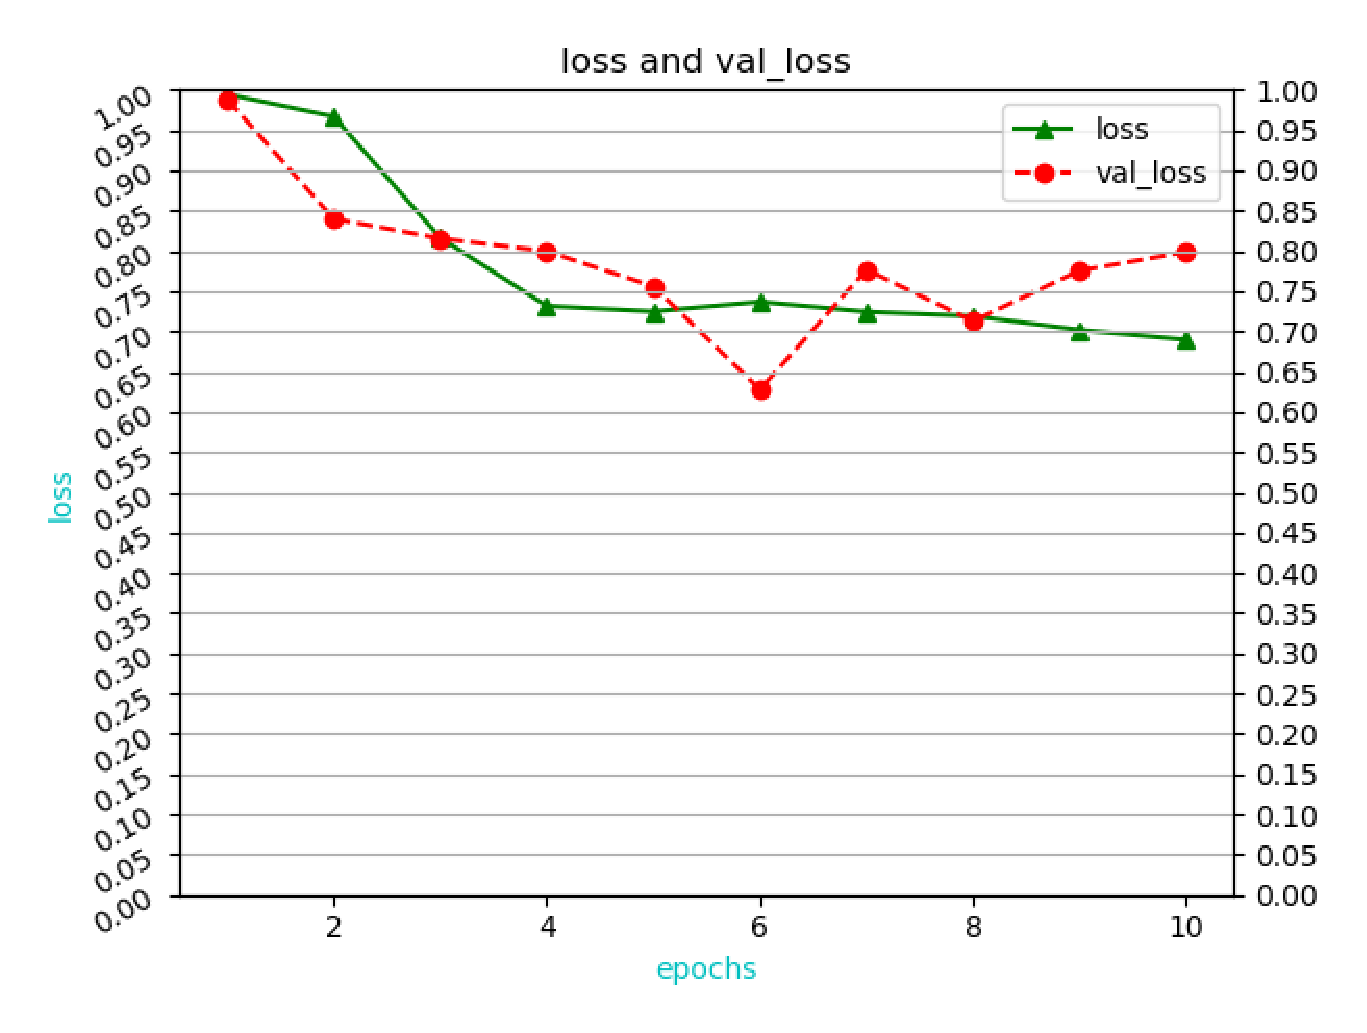
\includegraphics{body/model_pic/loss1}
\caption{}
\end{figure}

\begin{figure}
\centering
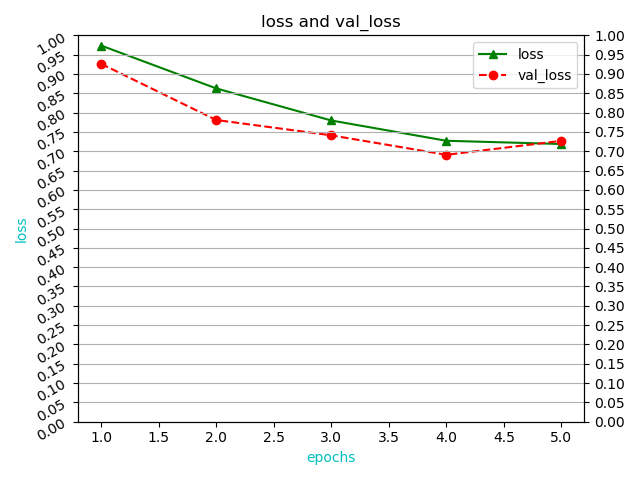
\includegraphics{body/model_pic/loss2}
\caption{}
\end{figure}

轮数:由loss图像所得,设置为5。

\subsection{选择次数(一轮中训练的次数)}

次数:次数=样本数/个数。

\subsection{选择个数(一次训练的样本数)}

个数:由于16张图片内存过大,而2张图片效果较差,所以设置为4。
